% !TeX spellcheck = en_GB
%%%%%%%%%%%%%%%%%%%%%%%%%% phdsymp_sample2e.tex %%%%%%%%%%%%%%%%%%%%%%%%%%%%%%
%% changes for phdsymp.cls marked with !PN
%% except all occ. of phdsymp.sty changed phdsymp.cls
%%%%%%%%%%                            %%%%%%%%%%%%%
%%%%%%%%%%  More information: see the header of phdsymp.cls  %%%%%%%%%%%%%
%%%%%%%%%%                            %%%%%%%%%%%%%
%%%%%%%%%%%%%%%%%%%%%%%%%%%%%%%%%%%%%%%%%%%%%%%%%%%%%%%%%%%%%%%%%%%%%%%%%%%%%%%


%\documentclass[10pt]{phdsymp} %!PN
\documentclass[twocolumn]{phdsymp} %!PN
%\documentclass[12pt,draft]{phdsymp} %!PN
%\documentstyle[twocolumn]{phdsymp}
%\documentstyle[12pt,twoside,draft]{phdsymp}
%\documentstyle[9pt,twocolumn,technote,twoside]{phdsymp}

\usepackage[english]{babel}    % Voor nederlandstalige hyphenatie (woordsplitsing)

\usepackage{graphicx}          % Om figuren te kunnen verwerken
\usepackage{graphics}			% Om figuren te verwerken.

\graphicspath{images/}

\usepackage{times}

\hyphenation{}

\def\BibTeX{{\rm B\kern-.05em{\sc i\kern-.025em b}\kern-.08em
  T\kern-.1667em\lower.7ex\hbox{E}\kern-.125emX}}

\newtheorem{theorem}{Theorem}

\begin{document}

\title{The user perceived performance of route planning APIs} %!PN

\author{Bert Marcelis}

\supervisor{Prof. dr. ir. Ruben Verborgh, Pieter Colpaert, Julian Andres Rojas Melendez}

\maketitle

\begin{abstract}

For the Web architectures behind route planning applications, remote procedure calls are commonplace, in which a server calculates the routes for all end-users.
Linked Connections introduces an alternative architecture following the REST constraints, publishing the raw data in fragments.
While benchmarks show a higher cost-efficiency of Linked Connections on the server, it is currently not known how it performs on clients, that now also need to execute the route planning algorithm.
In this work, we study the user-perceived performance of route planning on the client-side, consuming more bandwidth, versus route planning on the server-side. 
An isomorphic app was developed with both route planning on the client-side as on the server-side.
Both technical performance and user-perceived performance were tested among 17 travelers, and 81 respondents gave insights on their use of travel companions.

We found that the performance of Linked Connections heavily depends on the type of information, the query and the user’s device. Linked Connections can be faster or slower than a query answering API based on these parameters. 
The value of offline searches outweighs the slower experience for most users.
For a majority of the users, the benefit of offline searches outweighs the slower speed of Linked Connections. Even though Linked Connections is slower than the reference API, users consider it, on recent devices, as fast as their default application.

\end{abstract}

\begin{keywords}
Linked Connections, public transport
\end{keywords}

\section{Introduction}
\PARstart{P}{ublic} transport is essential in every city. To make use of this transport, travellers frequently use their smartphones or websites to get route planning advice. The most common way to provide these applications and websites with data is by using Remote Procedure Call (RPC) APIs, in which case a server calculates the route or information a user needs, and serves the user with a personalized response. This approach is costly and depends on a continuous connection with the route planning server. Services which need to make queries in bulk, for example to construct insights and collect analytics, use the General Transport Format Specification (GTFS). In this case they can answer all queries themselves, but this method takes too much time and processing power to be applied in mobile end user devices.

Linked Connections tries to find a balance between these two approaches, and has already proven to be 75\% more cost-efficient~\cite{colpaert17}. While the server performance and costs have been researched, the performance and user-experience for a client based on Linked Connections is still unknown. This work will explore various aspects of the performance and user-experience by developing an isomorphic application to compare Linked Connections to a reference RPC API, which uses the same data and algorithms, but runs all calculations on the server. This will show if Linked Connections is a better format -- having a better user-perceived performance and user-experience -- compared to RPC APIs.

\section{State of the art}

Application for public transport are, at this time, commonly driven by RPC APIs. These APIs are based on dumb clients asking a smart server for an answer. On one hand this means it can be used on all clients, as it does not require much resources client-side. On the other hand it can be costly, as every response is personalized, the server has to do processor-intensive tasks and needs to be scaled according to the load. Other negative aspects are the requirements for a constant internet connection, and the fact that individual developers can't alter the route planning algorithm for their application.

When transport data is needed in bulk, for example when someone wants to gather statistics, GTFS can be used. While it is a resource-intensive task to deduce information from GTFS, it does not need API calls for every query. Unfortunately, due to GTFS being resource intensive, it's not fit for mobile devices or cases where results are needed quickly.

Linked connections tries to find a balance between these two technologies, by publishing the raw data in chronological, easy-to-use linked fragments. It's proven to be server efficient, and when load increases, performance increases instead of decreases~\cite{colpaert17}.

\section{User perceived performance of web architectures}

Every web architecture has specific properties, for example latency, performance, cache reuse, ...~\cite{verborgh16}. While these are all technical values, there is also the user-perceived performance. First defined by Roy T. Fielding~\cite{fielding99} as the latency between steady-states for a browser-based application, it comprises all processing needed, not only network traffic. For a (browser) application, the total latency consists of the following parts:
\begin{enumerate}
\item the time needed for the user agent to recognize the event that initiated the action
\item the time required to setup any interaction(s) between components
\item the time required to transmit each interaction to the components
\item the time required to process each interaction on those components
\item the time required to complete sufficient transfer before the user agent is able to begin rendering a usable result.
\item the time required to complete processing of the result of the interaction(s) before the user agent is able to begin rendering a usable result.
\end{enumerate}

While only steps 3,4 and 5 are directly dependent on network connectivity, all of theses steps can be influenced by the used architecture.

When not only focussing on performance, but also on the way users interact with technology, it is important to define the user-experience (UX). UX is a broad term, originally designating the design and usage of interfaces, making it a synonym for interactions and usability~\cite{avila11}, but it is also used for non-instrumental needs and experiences in a more complex way~\cite{avila11}. In this work UX will always be considered in this broader way.

\section{Evaluation design}

In order to evaluate Linked Connections and compare it to RPC APIs, an isomorphic application is developed. This application allows to test Linked Connections and an RPC API, while keeping the user interface and client-side logic identical. An RPC API is developed to be used as a reference for Linked Connections. It is backed by the same data and algorithms as the client-side Linked Connections implementation, thus allowing for a fair comparison. As a result, the only difference is which entity does the processing, and how data is transported.

Using this application, user testing is conducted on 17 test persons. Each tester is asked to search for data he usually searches for, one time using the reference RPC API as data provider, and using the Linked Connections implementation the second time. After testing and grading Linked Connections, they are also encouraged to turn off their network connection and test the offline capabilities using Linked Connections.
Users are only informed over differences between both implementations after the test has completed, as to not bias them. For each implementation, the user grades the speed of listing departures and arrivals for a station, journeys from A to B and vehicle trips. Users are also asked to compare each implementation to their currently used application. To conclude, they have to explicitly choose between both implementations regarding speed for each endpoint, and which implementation they favor the most, taking into account both speed and offline access. 

In order to know what's important to users, a survey is held under 81 travellers. This survey asks about past experiences, needs, mobile data, privacy, and concludes by shortly polling how interested respondents are in the features which can be offered by Linked Connections.

\section{Results}
\begin{figure}[ht]
	\begin{center}
		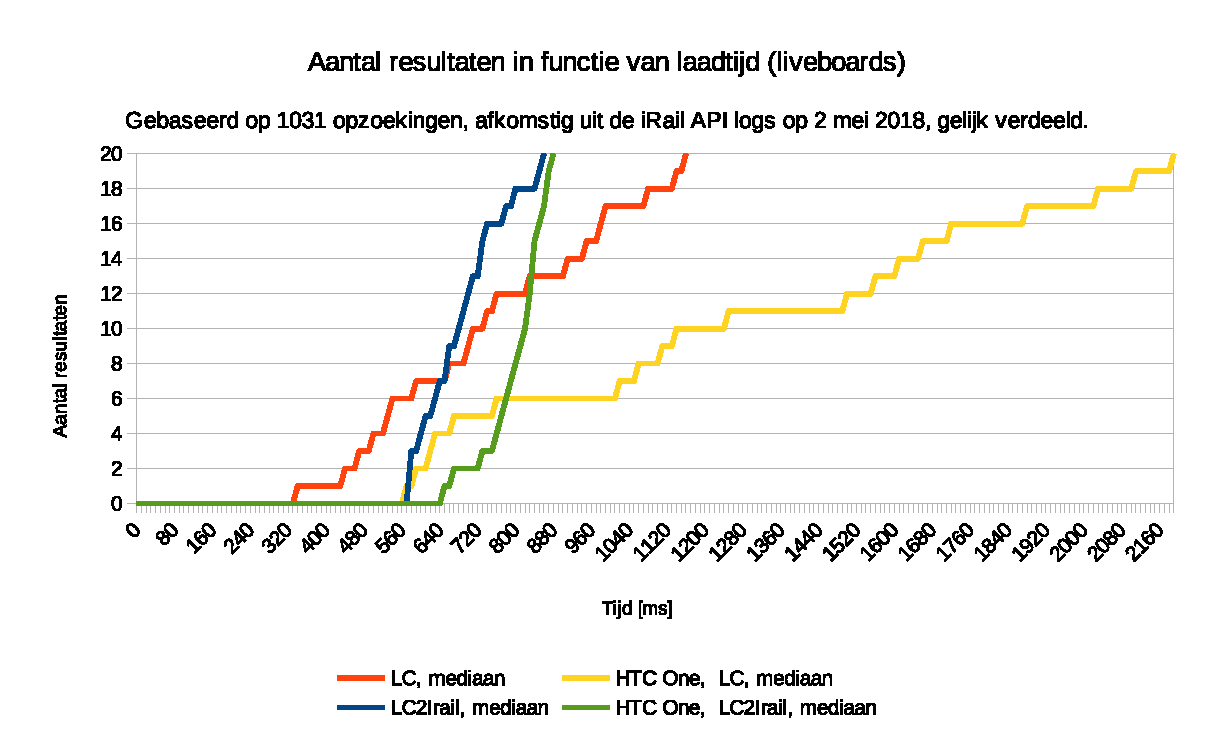
\includegraphics[width=.50\textwidth]{images/dief_liveboards_gemiddeld.eps}
		\caption{\label{fig:liveboard} }
	\end{center}
\end{figure}

\begin{figure}[ht]
	\begin{center}
		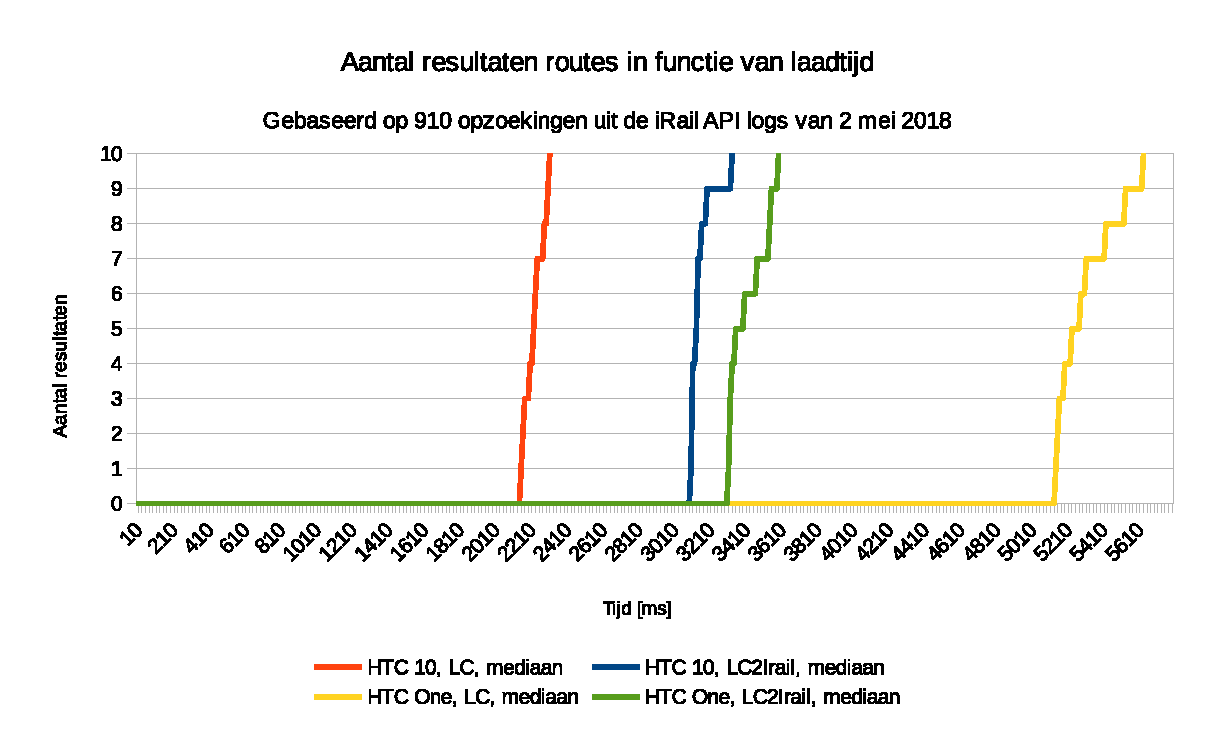
\includegraphics[width=.50\textwidth]{images/dief_routes_gemiddeld.eps}
		\caption{\label{fig:route} }
	\end{center}
\end{figure}

\begin{figure}[ht]
	\begin{center}
		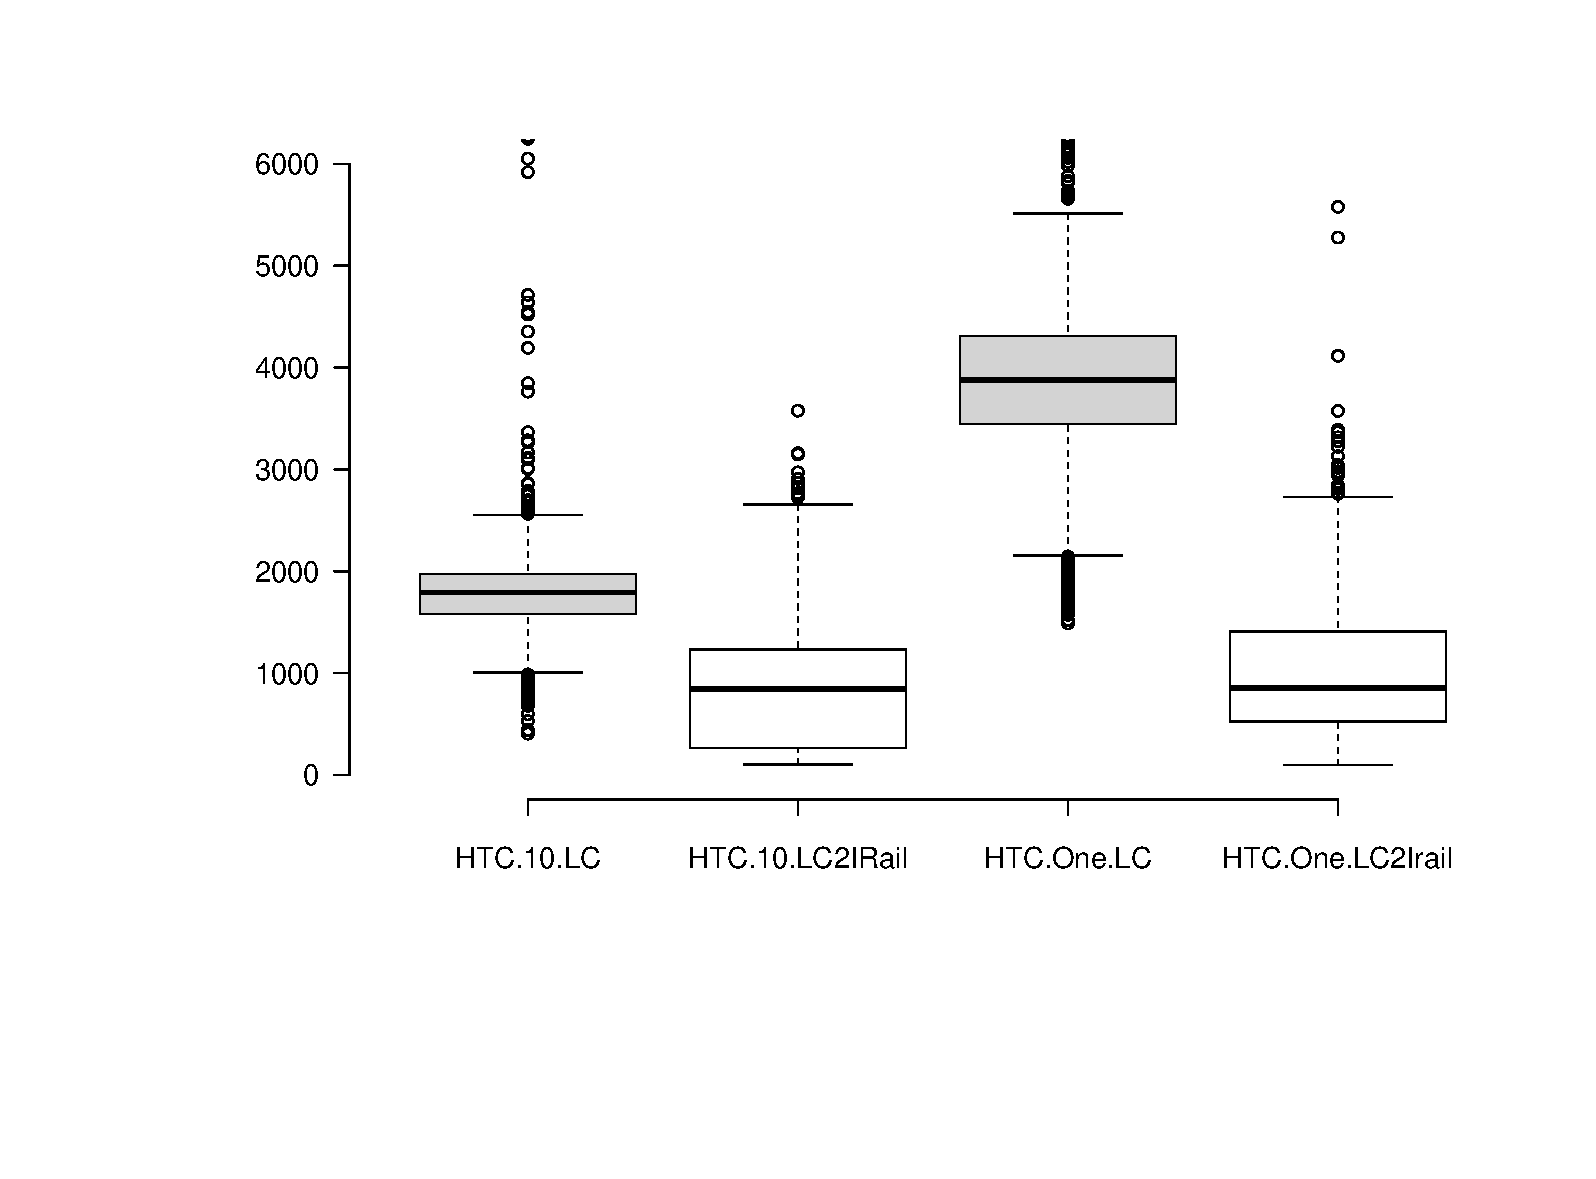
\includegraphics[trim=3cm 4cm 0 0, width=.50\textwidth]{images/boxplot_vehicles.eps}
		\caption{\label{fig:vehicle} }
	\end{center}
\end{figure}

\begin{figure}[ht]
	\begin{center}
		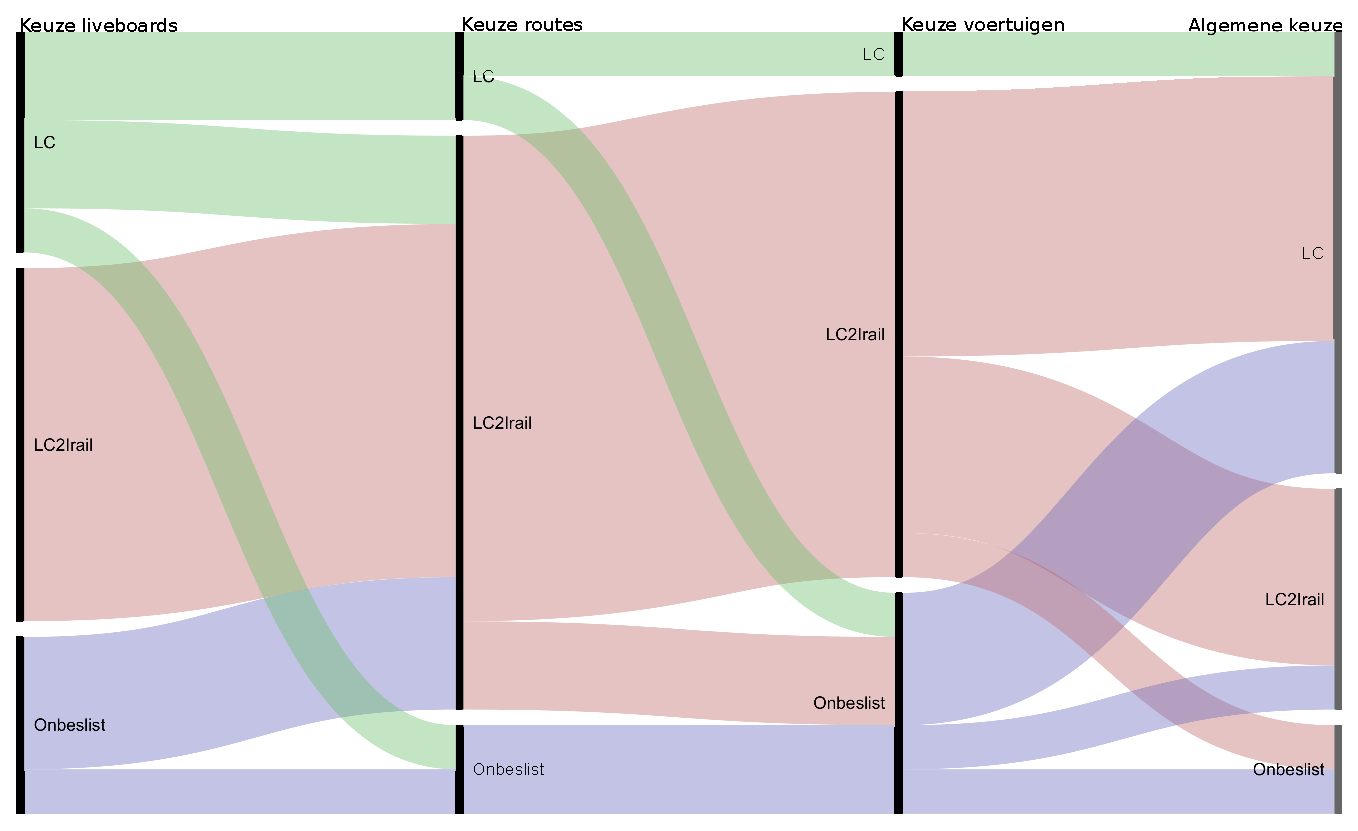
\includegraphics[width=.50\textwidth]{images/alluvial_user_choice.eps}
		\caption{\label{fig:choices} }
	\end{center}
\end{figure}

\section{Discussion}
 
\section{Conclusion}

\nocite{*}
\bibliographystyle{phdsymp}
%%%%%\bibliography{bib-file} % commented if *.bbl file included, as
%%%%%see below


%%%%%%%%%%%%%%%%% BIBLIOGRAPHY IN THE LaTeX file !!!!! %%%%%%%%%%%%%%%%%%%%%%%%
%% This is nothing else than the phdsymp_sample2e.bbl file that you would%%
%% obtain with BibTeX: you do not need to send around the *.bbl file    
%%
%%---------------------------------------------------------------------------%%
%
\begin{thebibliography}{1}
\bibitem{colpaert17}
\bibitem{fielding99}
\bibitem{avila11}
\bibitem{verborgh16}
\end{thebibliography}
%
%%---------------------------------------------------------------------------%%

\end{document}

%%%%%%%%%%%%%%%%%%%%% End of phdsymp_sample2e.tex %%%%%%%%%%%%%%%%%%%%%%%%%%%
